% https://www.wolfdynamics.com/training/OF_WS2020/traning_session2020.pdf
\subsection{Método de los volúmenes finitos}

\begin{frame}
	El problema del método de diferencias finitas es que la información
	que tiene en cuenta solo está formada por los valores que toma la
	función $U$ en diferentes puntos del espacio, lo que hace que la
	información que se sitúa entre estos puntos de discretización se
	pierda (vea la Figura~\ref{fig:discretization}).
	El método de los volúmenes finitos soluciona esto considerando toda
	la información, pero en forma promediada, contenida entre dos nodos.

	\begin{figure}[ht!]
		\centering
		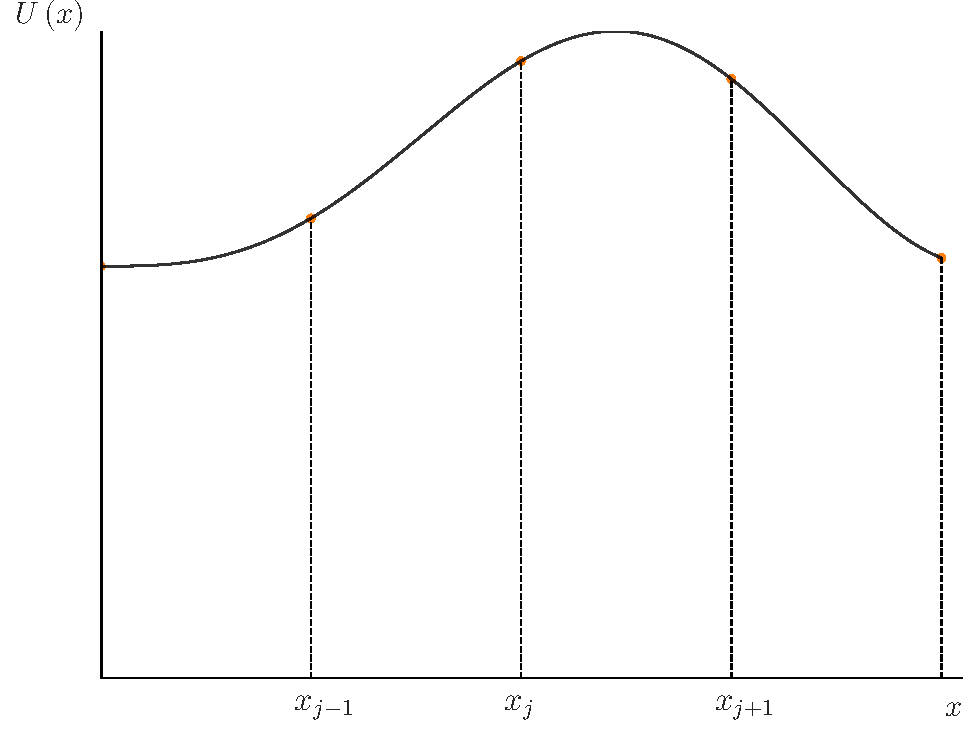
\includegraphics[width=.45\paperwidth]{discretization}
		\caption{Discretización de una función.}
		\label{fig:discretization}
	\end{figure}

	Para esto, el método de volúmenes finitos se reduce a la forma
	conservativa de la ecuación a resolver, luego discretiza los flujos
	para determinar la evolución del sistema.
	Por ejemplo, considere una \emph{ley de conservación} sujeto a
	condiciones iniciales y/o de fronteras.

	\begin{equation}\label{eq:conservationlaw}
		\diffp{U}{t}+
		\diffp{
			f
			\left(U\right)
		}{x}=
		0
	\end{equation}

	\begin{alertblock}\leavevmode
		\begin{enumerate}
			\item

			      Si el flujo
			      \begin{math}
				      f
				      \left(U\right)=
				      cU
			      \end{math}
			      es \emph{advectivo}, entonces~\eqref{eq:conservationlaw} es
			      la ecuación de advección lineal~\eqref{eq:advectionPDE}.

			\item


			      Si el flujo
			      \begin{math}
				      f
				      \left(U\right)=
				      -\alpha\diffp{U}{x}
			      \end{math}
			      es \emph{difusivo}, entonces~\eqref{eq:conservationlaw} es
			      la ecuación de difusión lineal~\eqref{eq:diffusion1d}.

			\item

			      Si el flujo
			      \begin{math}
				      f
				      \left(U\right)=
				      cU-
				      \alpha\diffp{U}{x}
			      \end{math},
			      entonces~\eqref{eq:conservationlaw} es la ecuación de
			      advección-difusión lineal~\eqref{eq:advection-diffusion1d}.
		\end{enumerate}
	\end{alertblock}
\end{frame}

\begin{frame}

	Integramos esta ecuación (para encontrar su ``forma conservativa'')
	en un volumen de control, que en dimensión $1$ es solo un segmento
	centrado alrededor de
	\begin{math}
		x_{j}=
		j\Delta x
	\end{math},
	donde $\Delta x$ es el tamaño de las celdas de la malla.
	Los extremos de este segmento son $x_{j-\frac{1}{2}}$ y
	$x_{j+\frac{1}{2}}$; aquí el índice $\frac{1}{2}$ nos dice que estos
	dos puntos están en la interfaz con celdas vecinas centradas en
	$x_{j-1}$ y $x_{j+1}$.
	En lugar de considerar como antes el valor tomado por $U$ en $x=x_{j}$,
	introducimos el valor promedio de $U$ en el segmento
	\begin{math}
		\mathcal{C}_{j}=
		\left[
			x_{j-\frac{1}{2}},
			x_{j+\frac{1}{2}}
			\right]
	\end{math}:

	\begin{equation*}
		U^{n}_{j}=
		\dfrac{1}{\Delta x}
		\int_{\mathcal{C}_{j}}
		U
		\left(x,t^{n}\right)
		\dl x.
	\end{equation*}

	\begin{figure}[ht!]
		\centering
		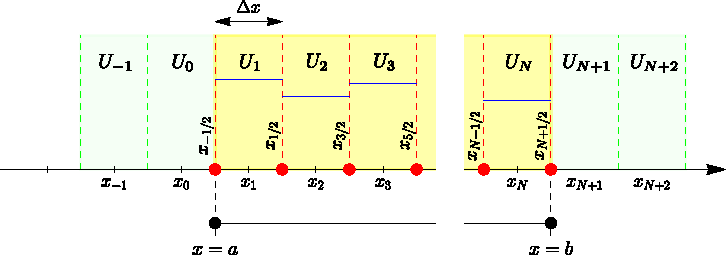
\includegraphics[width=.5\paperwidth]{computationalgrid}
		\caption{Malla computacional.
			El área de color amarillo representa el dominio computacional
			$\left[a,b\right]$, mientras que el área de color verde
			representa el dominio extendido para manejar las condiciones de
			frontera.
			El dominio computacional se puede extender mediante la inclusión
			de \emph{celdas fantasmas}.
		}
		\label{fig:piecewise}
	\end{figure}
\end{frame}

\begin{frame}
	\begin{figure}[ht!]
		\centering
		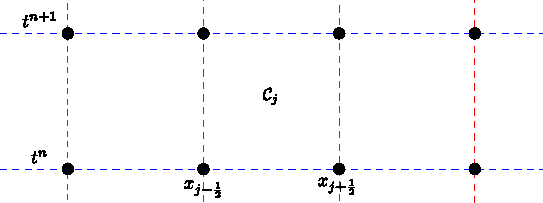
\includegraphics[width=.5\paperwidth]{computationaldomainfinitevolume}
		\caption{Dominio computacional y la malla en el plano $x-t$.}
		\label{fig:computationaldomainfinitevolume}
	\end{figure}

	La ventaja de esta discretización frente a las técnicas de
	diferencias finitas es que el método es \emph{conservativo}, es
	decir, los flujos (que expresan balances de masa, cantidad de
	movimiento, etc.) se describen correctamente.

	\begin{figure}[ht!]
		\centering
		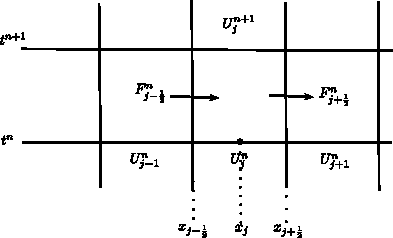
\includegraphics[width=.5\paperwidth]{finitevolumediagram}
		\label{fig:finitevolumediagram}
		\caption{Plano $x-t$ y el flujo entre las celdas.}
	\end{figure}

	Integramos~\eqref{eq:conservationlaw} sobre el volumen de control
	\begin{math}
		\left[
			x_{j-\frac{1}{2}},
			x_{j+\frac{1}{2}}
			\right]\times
		\left[
			t^{n},
			t^{n+1}
			\right]
	\end{math}.
	Comencemos integrando con respecto a la variable espacial $x$.
	Como la cuadrícula es fija podemos invertir las operaciones de
	diferenciación:

	\begin{equation*}
		\int_{C_{j}}
		\diffp{U}{t}
		\dl x=
		\diffp{}{t}
		\int_{\mathcal{C}_{j}}
		U\dl x.
	\end{equation*}

	También tenemos:

	\begin{equation*}
		\int_{\mathcal{C}_{j}}
		\diffp{U}{x}
		f\left(U\right)
		\dl x+
		{
		\left[
			f\left(U\right)
			\right]
		\Bigr|
		}_{x_{j-\frac{1}{2}}}^{x_{j+\frac{1}{2}}}
		=0.
	\end{equation*}

	Por tanto, la integración de~\eqref{eq:conservationlaw} sobre
	$\mathcal{C}_{j}$ es

	\begin{equation*}
		\diff{}{t}
		\int_{\mathcal{C}_{j}}
		U\left(x,t\right)
		\dl x=
		f\left(U\left(x_{j-\frac{1}{2}},t\right)\right)-
		f\left(U\left(x_{j+\frac{1}{2}},t\right)\right).
	\end{equation*}

	Una integración con respecto al tiempo entre los tiempos $t^{n}$ y
	$t^{n+1}$ proporciona la ecuación

	\begin{equation*}
		\int_{\mathcal{C}_{j}}
		U
		\left(x,t^{n+1}\right)
		\dl x-
		\int_{\mathcal{C}_{j}}
		U
		\left(x,t^{n}\right)
		\dl x=
		\int_{t^{n}}^{t^{n+1}}
		\left[
			f\left(U\left(x_{j-\frac{1}{2}},t\right)\right)-
			f\left(U\left(x_{j+\frac{1}{2}},t\right)\right)
			\right]\dl t,
	\end{equation*}

	que también se puede escribir en la forma

	\begin{equation*}
		\boxed{
			U^{n+1}_{j}=
			U^{n}_{j}-
			\frac{\Delta t}{\Delta x}
			\left(
			F^{n}_{j+\frac{1}{2}}-
			F^{n}_{j-\frac{1}{2}}
			\right),
		}
	\end{equation*}

	donde introdujimos el flujo promedio (a lo largo del tiempo)

	\begin{equation*}
		F^{n}_{j\pm\frac{1}{2}}=
		\frac{1}{\Delta t}
		\int_{t^{n}}^{t^{n+1}}
		f\left(U\left(x_{j\pm\frac{1}{2}}\right),t\right)
		\dl t,
	\end{equation*}

	con tamaño de paso temporal $\Delta t=t^{n+1}-t^{n}$.
	Todo el desafío de los MVF será encontrar una aproximación del flujo
	promedio
	\begin{math}
		F^{n}_{j+\frac{1}{2}}
	\end{math}
	en la interfaz entre dos celdas (vea la
	Figura~\ref{fig:computationaldomainfinitevolume}).
	Uno de los MVF es el esquema de \emph{Lax-Friedrichs}, que consiste
	en definir una función de flujo numérico de la siguiente manera:

	\begin{equation*}
		F^{n}_{j+\frac{1}{2}}=
		\frac{1}{2}
		\left[
			f\left(U^{n}_{j+1}\right)-
			f\left(U^{n}_{j}\right)-
			\frac{\Delta x}{\Delta t}
			\left(
			U^{n}_{j+1}-
			U^{n}_{j}
			\right)
			\right].
	\end{equation*}
\end{frame}

\begin{frame}
	Este esquema es similar a una discretización numérica de la ecuación
	de advección no lineal con un término difusivo

	\begin{equation*}
		\diffp{U}{t}+
		\diffp{f\left(U\right)}{x}=
		\beta
		\diffp[2]{U}{x},
	\end{equation*}

	con
	\begin{math}
		\beta=
		\frac{{\left(\Delta x\right)}^{2}}{2\Delta t}
	\end{math}.

	El término difusivo adicional comparado con la ecuación
	original~\eqref{eq:conservationlaw} sirve para estabilizar la
	solución numérica, sirviendo aquí la difusión para atenuar cualquier
	inestabilidad que aparecería.

	Posteriormente veremos esquemas que son mucho más eficientes que el
	esquema Lax-Friedrichs, que introduce demasiada difusión numérica.
	Estos esquemas explotan características específicas de las ecuaciones
	hiperbólicas, en particular el shock y la propagación de información.

	Consideremos una ecuación hiperbólica en una dimensión espacial y en
	su forma conservativa.

	\begin{equation}\label{eq:hyperbolic1d}
		\diffp{\bm{U}}{t}+
		\diffp{\bm{f}\left(\bm{U}\right)}{t}=
		0,
	\end{equation}

	donde $U\in\mathbb{R}^{m}$ y $\bm{f}$ es la función flujo.

	Consideramos una cuadrícula uniforme sobre un intervalo
	$\left[a,b\right]$ dividida en $N$ celdas idénticas de tamaño
	\begin{math}
		\Delta x=
		\dfrac{b-a}{N}
	\end{math}.

	Los centros de las celdas se denotan por $x_{j-\frac{1}{2}}$

	\begin{equation*}
		x_{j}=
		a+
		\left(
		j-
		\frac{1}{2}
		\right)
		\Delta x.
	\end{equation*}

	Definimos la celda
	\begin{math}
		\mathcal{C}_{i}=
		\left[
			x_{j-\frac{1}{2}},
			x_{j+\frac{1}{2}}
			\right]
	\end{math},
	centrada alrededor de la celda $x_{j}$ y cuyos límites (o interfaces)
	son $x_{j\pm\frac{1}{2}}$.
	Note que
	\begin{equation*}
		x_{-\frac{1}{2}}=
		a,
		\quad
		x_{N+\frac{1}{2}}=
		b.
	\end{equation*}

	El tamaño de paso es denotado por $\Delta t=t^{n+1}-t^{n}$.
	El dominio computacional es $\left[a,b\right]$

	\begin{equation*}
		\int_{
			x_{j-\frac{1}{2}}
		}^{
			x_{j+\frac{1}{2}}
		}
		\diffp{\bm{U}}{t}
		\dl x+
		\left[
			\bm{f}
			\left(\bm{U}\right)
			\right]
		=0.
	\end{equation*}
\end{frame}

\begin{frame}
	Integrating this equation again over
	\begin{math}
		\left(
		t_{n},
		t_{n+1}
		\right]
	\end{math}
	gives:

	\begin{equation*}
		\int_{
			x_{j-\frac{1}{2}}
		}^{
			x_{j+\frac{1}{2}}
		}
		\left(
		U
		\left(x,t^{n+1}\right)-
		U
		\left(x,t^{n}\right)
		\right)
		\dl x+
		\int_{t^{n}}^{t^{n+1}}
		\left[
			\bm{f}
			\left(\bm{U}\right)
			\right]
		\dl t=
		0.
	\end{equation*}

	\begin{equation*}
		U^{n}_{i}=
		\frac{1}{\Delta x}
		\int_{
			x_{j-\frac{1}{2}}
		}^{
			j+\frac{1}{2}
		}
		\bm{U}
		\left(x,t^{n}\right)
		\dl x.
	\end{equation*}

	\begin{equation*}
		\bm{F}^{n}_{j\pm\frac{1}{2}}=
		\frac{1}{\Delta t}
		\int_{t^{n}}^{t^{n+1}}
		\bm{f}
		\left(\bm{U}\left(x_{j\pm\frac{1}{2}}\right),t\right)
		\dl t.
	\end{equation*}

	Posteriormente veremos esquemas que son mucho más eficientes que el
	esquema Lax-Friedrichs (LxF), que introduce demasiada difusión
	numérica.
	Estos esquemas explotan las características específicas de las
	ecuaciones hiperbólicas, en particular el shock y la propagación de
	información.
\end{frame}

\subsubsection*{Esquema de Godunov}

\begin{frame}
	A finales de la década de $1950$,
	Godunov\footnote{Sergei Konstantinovich Godunov~(1929-2023) fue un
		matemático miembro de la Academia de Ciencias de Rusia y profesor
		del Instituto Sobolev de Matemáticas de Novosibirsk.
		El mayor avance realizado por Godunov fue proponer un método
		compatible con la propagación de discontinuidades.} propuso un
	algoritmo para resolver sistemas EDPs lineales hiperbólicas.
	La idea básica explotada por Godunov es

	\begin{description}
		\item[Reconstrucción]

		      Asuma que podemos aproximar la solución
		      \begin{math}
			      U
			      \left(x,t\right)
		      \end{math}
		      por una función constante a trozos
		      \begin{math}
			      \widetilde{U}^{n}_{j}
			      \left(x,t^{n}\right)=
			      U^{n}_{j}
		      \end{math}
		      en $x\in\mathcal{C_{i}}$.
		      %del dominio de cálculo y en el tiempo $t^n$, a
		      % partir de los valores promedio de las celdas
		      % (obtenidos en el paso 3 de promediar en $t^{n}$).
		      La más sencilla es considerar funciones constantes por partes
		      (esquema de Godunov de primer orden):

		      \begin{align*}
			      U^{n}_{j}
			       & =
			      \frac{1}{\Delta x}
			      \int_{x_{i-\frac{1}{2}}}^{i+\frac{1}{2}}
			      \widetilde{U}
			      \left(x,t^{n}\right)
			      \dl x, \\
			       & =
			      \frac{1}{\Delta x}
			      \int_{x_{i}-\frac{\Delta x}{2}}^{x_{i}+\frac{\Delta x}{2}}
			      \left[
				      \widetilde{U}
				      \left(x_{j},t^{n}\right)+
				      \left(x-x_{i}\right)
				      \diffp{U\left(x_{j},t^{n}\right)}{x}+
				      \frac{{\left(x-x_{j}\right)}^{2}}{2}
				      \diffp[2]{U\left(x_{j},t^{n}\right)}{x}
				      \right]
			      \dl x. \\
			       & =
			      U\left(x_{j},t^{n}\right)+
			      \frac{{\left(\Delta x\right)}^{2}}{24}
			      \diffp[2]{U\left(x_{j},t^{n}\right)}{x}
		      \end{align*}

		      % para
		      % \begin{math}
		      %   x_{j-\frac{1}{2}}\leq
		      %   x\leq
		      %   x_{j+\frac{1}{2}}
		      % \end{math}.
		      Esto nos permite considerar que en cada paso de tiempo y en cada interfaz entre dos celdas,
		      resolvemos un problema de Riemann.
		      Naturalmente, es posible considerar formas de reconstrucción más complejas,
		      por ejemplo considerando funciones lineales por partes.
		      Esto es lo que se hace con los llamados \emph{métodos de alta resolución}.

		\item[Evolución]

		      Propagación de las discontinuidades en las interfaces $x_{j-\frac{1}{2}}$ tomando como condición inicial los valores
		      \begin{math}
			      \widetilde{U}
			      \left(x,t^{n}\right)
		      \end{math}.
		      Por ejemplo, podemos utilizar el método descrito en la ecuación (3.3). Deducimos U (x, tn+1):

		\item[Promedio]

		      Promediar las funciones alteradas por el paso de las discontinuidades

		      \begin{equation*}
			      U^{n+1}_{j}=
			      \frac{1}{\Delta x}
			      \int_{x_{i-\frac{1}{2}}}^{x_{i+\frac{1}{2}}}
			      \widetilde{U}
			      \left(x,t^{n+1}\right)
			      \dl x.
		      \end{equation*}
	\end{description}
\end{frame}

\begin{frame}
	\begin{figure}[ht!]
		\centering
		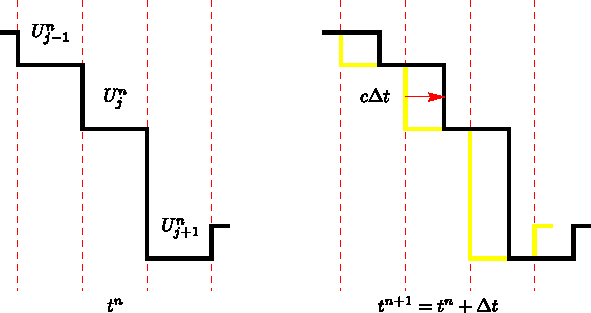
\includegraphics[width=.5\paperwidth]{piecewise}
		\caption{Advección de una función continua por partes.
		En el tiempo $t^{n}$, la función constante a trozos con valor $U^{n}_{j}$ en la celda $\mathcal{C}_{j}$.
		En el tiempo $t^{n+1}$, la función se ha desplazado en $c\Delta t$.
		El valor $U^{n+1}_{j}$ se obtiene promediando espacialmente desplazada en la celda $\mathcal{C}_{j}$.
		El problema puede interpretarse como la propagación de discontinuidades que se originan en el extremo
		$x_{j-\frac{1}{2}}$.
		Estas discontinuidades forman la onda $W_{i-\frac{1}{2}}=U_{j}-U_{j-1}$.}
		\label{fig:piecewise}
	\end{figure}

	Ahora veremos los principales tipos de ecuaciones diferenciales
	parciales que se encuentran en hidráulica:

	\begin{equation*}
		a_{j}=
		\dfrac{U^{n}_{j+1}-U^{n}_{j-1}}{2\Delta x}
	\end{equation*}

	\begin{equation*}
		a_{i}=
		\dfrac{U^{n}_{j}-U^{n}_{j-1}}{\Delta x}
	\end{equation*}

	\begin{equation*}
		a_{i}=
		\dfrac{U^{n}_{j+1}-U^{n}_{j}}{\Delta x}.
	\end{equation*}

	\begin{equation*}
		a_{i}=
		\operatorname{minmod}
		\left(
		\dfrac{U^{n}_{j}-U^{n}_{j-1}}{\Delta x},
		\dfrac{U^{n}_{j+1}-U^{n}_{j}}{\Delta x}
		\right)
	\end{equation*}
	Por fenṕmenos
	\begin{itemize}
		\item

		      transporte por convección (o advección);

		\item

		      transporte por difusión;

		\item

		      fenómenos ondulatorios;

		\item

		      fenómenos de equilibrio.
	\end{itemize}
\end{frame}
